\chapter{Implementation of a combined PCI-interferometer on \diiid}
\label{ch:Implementation}


\section{Optical-diagnostic access on \diiid}
\label{sec:Implementation:d3d_ports}
\diiid \space provides optical access to its plasmas
through a number of ports, as indicated in
Fig.~\ref{fig:Implementation:d3d_port_locations}.
The ports are labeled according to their
toroidal positions and their sightlines, and
an experimentalist should have at least
a rough familiarity with these conventions.
The toroidal location of a port
is given in degrees clockwise from ``machine north''
when viewing the machine from above
(note that machine north does \emph{not} correspond
to geographic or magnetic north).
The angular separation of adjacent toroidal ports is $15^{\circ}$.
Port sightlines can be vertical or radial.
Ports with vertical (V) sightlines
are labeled sequentially in terms of increasing major radius,
with $V1$ having the smallest major radius and
$V3$ having the largest major radius.
Radial ports (R) have sightlines
that are roughly aligned with the plasma's minor radius, and
they are labeled according to their positions
relative to the plasma midplane:
R0 sits at the plasma midplane,
R+1 and R+2 are the first and second ports
\emph{above} the plasma midplane, respectively, and
R-1 and R-2 are the first and second ports
\emph{below} the plasma midplane, respectively.

\begin{figure}
  \centering
  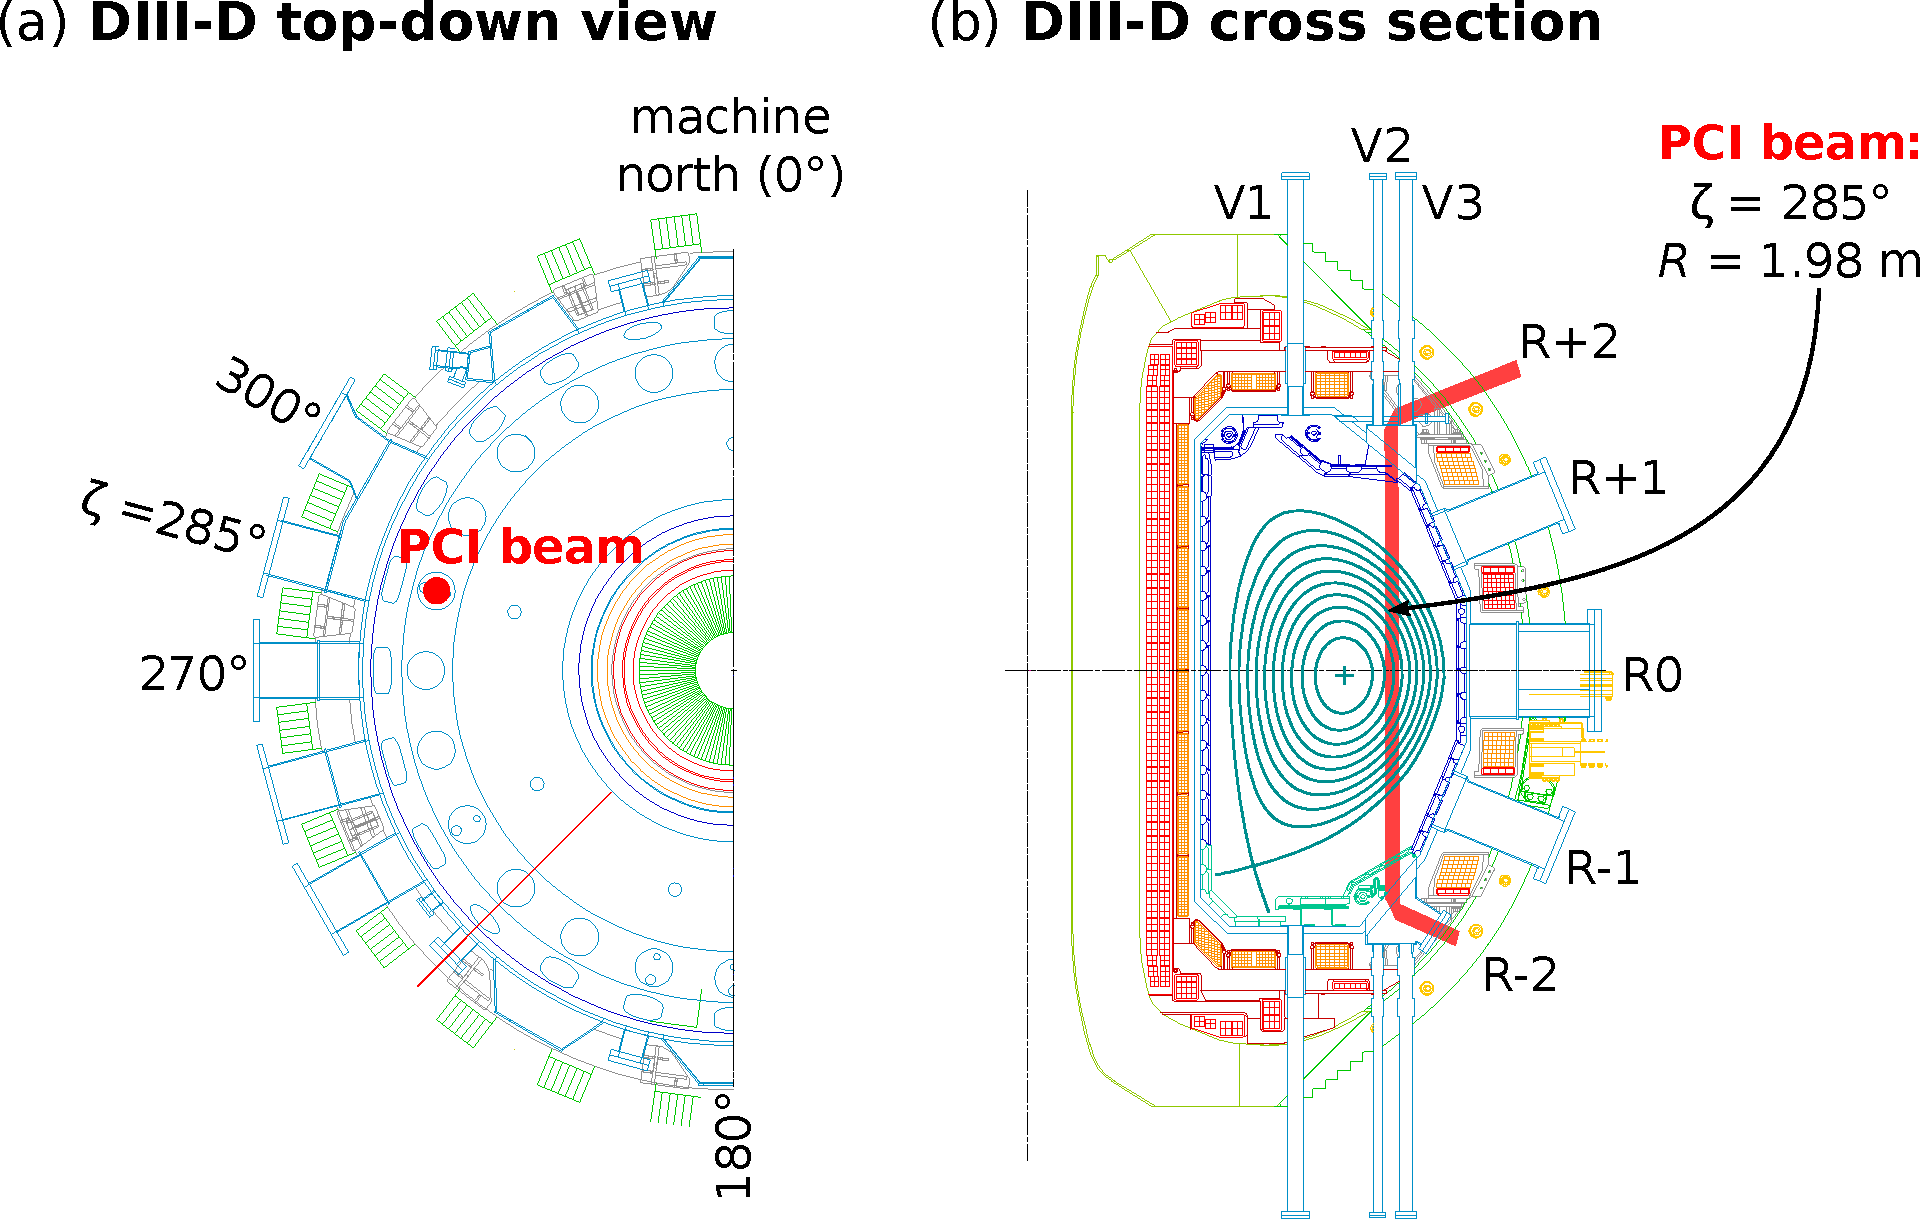
\includegraphics[width = \textwidth]{%
    Chapters/Implementation/figs/d3d_port_locations.pdf}
  \caption[\diiid \space port-labeling conventions and location of PCI]{%
    (a) View of \diiid \space from above,
    indicating the toroidal-labeling convention.
    (b) View of \diiid \space cross section,
    indicating the labeling convention
    for vertical (V) and radial (R) sightlines.
    The PCI beam enters the vessel through the $285^{\circ}$ R+2 port,
    propagates vertically downwards through the plasma
    at a major radius of $R = \SI{1.98}{\meter}$, and
    exits the vessel through the $285^{\circ}$ R-2 port.}
\label{fig:Implementation:d3d_port_locations}
\end{figure}


\section{\diiid's pre-existing PCI system}
The \diiid \space PCI system is
thoroughly described elsewhere~\cite{dorris_rsi09, dorris_phd}, but
the system components of relevance to this work
are briefly summarized below for completeness.


\subsection{System geometry}
The system is currently configured
in the ``Phase II'' geometry~\cite{dorris_rsi09},
with the probe beam propagating vertically downwards
from the $285^{\circ}$ R+2 port to the $285^{\circ}$ R-2 port.
The beam center sits at $R = $ \SI{1.98}{\meter}.
Both the toroidal and radial positions
of the PCI beam are shown in
Fig.~\ref{fig:Implementation:d3d_port_locations}.

The PCI system's vertical beam path constrains
the types of fluctuations it can and cannot detect.
Namely, the PCI-measured intensity fluctuations
(\ref{eq:InterferometricMethods:pci_intensity})
correspond to \emph{line-integrated} electron-density fluctuations, which
are the physical origin of the phase fluctuations $\tilde{\phi}$ in
(\ref{eq:InterferometricMethods:phase_fluctuation}).
Because it is a line-integrated measurement,
only fluctuations propagating perpendicular to the beam path are detected,
as fluctuations propagating parallel to the beam path
are effectively averaged out of the signal
\graffito{\textcolor{red}{what about $\delta \omega$?}}
(and, at a more fundamental level, fluctuations propagating
parallel to the beam path do \emph{not} spatially scatter the probe beam).
\graffito{\textcolor{red}{citation? Wesson?}}
Now, electrostatic turbulence (e.g.\ ITG, ETG) tends to be field-aligned
such that $k_{\perp} \gg k_{||}$, where
the $\perp$ and $||$ subscripts are used here to indicate
orientations that are perpendicular to and parallel to
the local magnetic field, respectively.
To lowest order, then, electrostatic fluctuations propagate
perpendicular to a tokamak's toroidal field.
PCI's vertical beam path and
the field-aligned constraint of electrostatic turbulence
imply that PCI is predominantly sensitive to fluctuations
with finite major-radial wavenumber $k_R$.
Thus, PCI's 32-element, 1-dimensional detector array
is oriented in the image plane such that
each detector element corresponds to a unique major radius in the plasma.

In some situations, spatially filtering ``masks''
\cite{dorris_rsi09, dorris_phd, lin_rsi06} or
2-dimensional detector arrays
\cite{sanin_rsi04, tanaka_rsi16}
can be used to localize measurements
by exploiting the spatial variation
in the magnetic field's orientation along the beam path.
These localization techniques typically work best
for high-$k$ measurements.
Note that $k_R$ is related to the
theoretically relevant poloidal wavenumber $k_{\theta}$ via
\begin{equation}
  k_R = k_{\theta} \csc[\alpha(R, z)],
  \label{eq:Implementation:kR_to_ktheta}
\end{equation}
where $\alpha(R, z)$ is the angle
between the beam path and the local flux surface,
as shown schematically in
Fig.~\ref{fig:Implementation:relating_kR_to_ktheta}.
Of course, the fluctuation measurements must be localized,
either via direct measurement
(with 2-dimensional detector arrays or ``masks'')
or via inference from other plasma properties,
before (\ref{eq:Implementation:kR_to_ktheta})
can be inverted to yield $k_{\theta}$
from measured values of $k_R$.

\begin{figure}
  \centering
  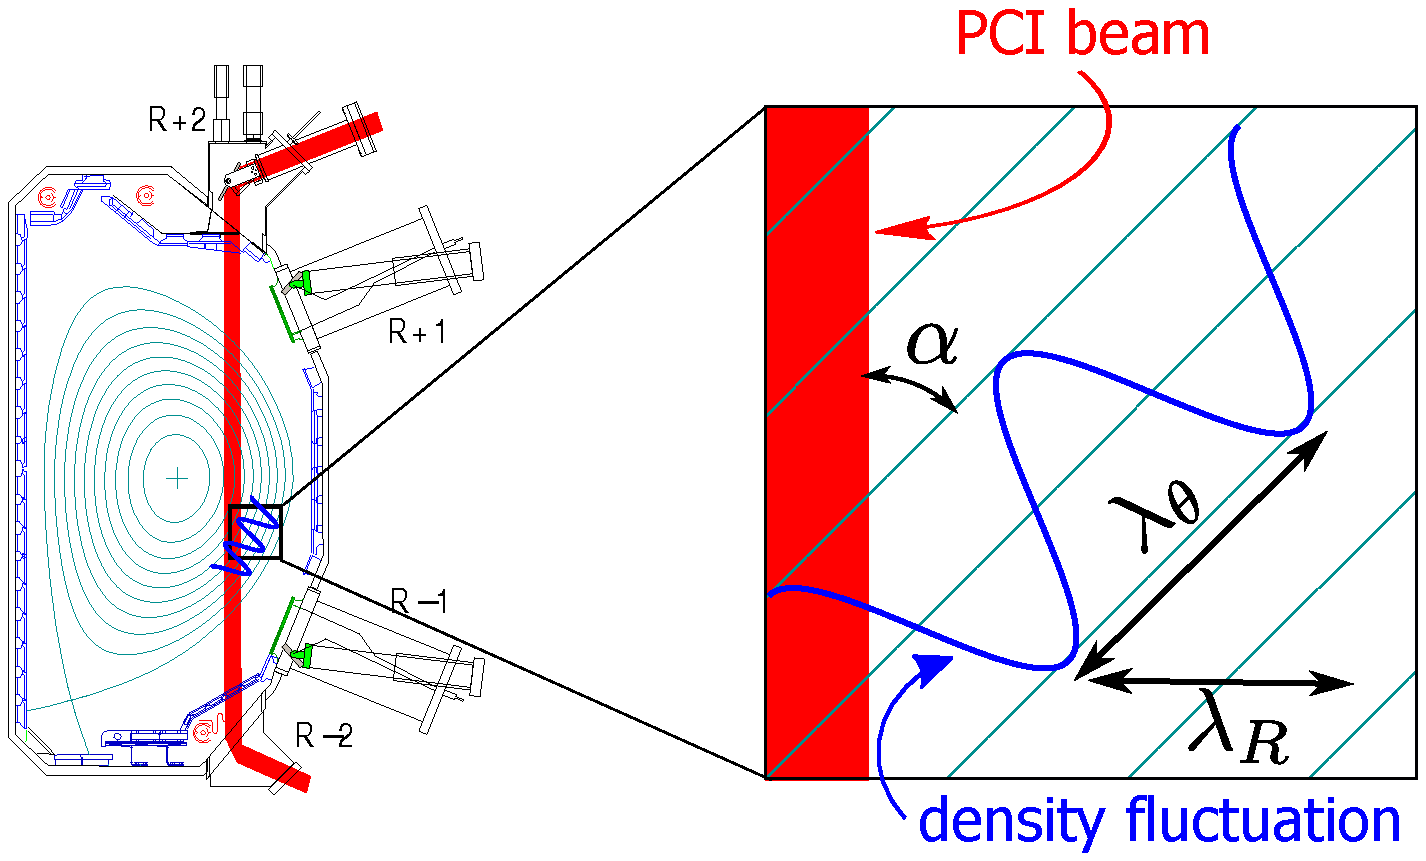
\includegraphics[width = 0.9 \textwidth]{%
    Chapters/Implementation/figs/kR_to_ktheta.pdf}
  \caption[Relating $k_R$ to $k_{\theta}$]{%
    The major-radial wavenumber $k_R = 2 \pi / \lambda_R$ and
    the poloidal wavenumber $k_{\theta} = 2 \pi / \lambda_{\theta}$
    are related via $\alpha(R, z)$, which
    is the angle between PCI's vertical probe beam and
    the local flux surface.}
\label{fig:Implementation:relating_kR_to_ktheta}
\end{figure}


\subsection{Spatial bandwidth}
Several critical wavenumbers were defined in
Section~\ref{sec:InterferometricMethods:pci} that
characterize the spatial bandwidth of a PCI system.
The goal of this section is to evaluate each of these
wavenumbers with the relevant parameters from
the \diiid \space PCI system.

PCI's low-$k$ cutoff, $k_g$, is physically constrained by
the free-space diffraction of the in-vessel probe beam.
This constraint was derived both
by examining the far-field overlap of the scattered and unscattered beams as in
(\ref{eq:InterferometricMethods:kmin_for_far_field_beam_separation}) and
by matching the focal-plane spot size of the unscattered beam
with the width of the phase-plate groove as in
(\ref{eq:InterferometricMethods:pci_kmin_physics}).
Both approaches yield the identical constraint that
$k_g^{\text{min}} = 2 / w_0$, where
$w_0$ is the 1/e $E$ radius of the in-vessel probe beam.
The maximum value of $w_0$ is set by the aperture diffraction criterion
(\ref{eq:DesignConsiderations:summary:aperture_radius_for_minimal_diffraction}).
After beam expansion and collimation,
the $4"$-diameter $285^{\circ}$ R+2 port window
is the smallest aperture seen by the beam
prior to its interaction with the plasma.
To satisfy the aperture diffraction criterion
(\ref{eq:DesignConsiderations:summary:aperture_radius_for_minimal_diffraction})
with this $4"$-diameter window,
the expansion optics are configured to produce a collimated beam with
$w_0 = 4/3" \approx \SI{3.4}{\centi\meter}$,
corresponding to
\begin{equation}
  k_g^{\text{min}} \approx \SI{0.6}{\per\centi\meter}.
  \label{eq:Implementation:kg_min}
\end{equation}

PCI's \emph{realized} low-$k$ cutoff, however,
is typically $\sim 2-3 \times$ larger than
the diffraction-limited $k_g^{\text{min}}$.
This occurs if the width of the phase-plate groove is oversized
relative to the unscattered beam's focal-plane spot size.
In such situations the realized low-$k$ cutoff is given by
(\ref{eq:InterferometricMethods:pci_kmin_engineering}).
Despite sacrificing some of the system's low-$k$ range,
operating with an oversized phase-groove width can be advantageous
on large, vibration-prone fusion experiments.
To see this, recall that the phase groove typically reflects
only a fraction $\eta < 1$ of the incident unscattered beam power
(the forward-facing surface of the \diiid\space phase-plate groove
is uncoated ZnSe, which has $\eta = 0.17$ at $\SI{10.6}{\micro\meter}$);
if vibration-induced misalignments
push the unscattered beam out of the phase groove,
there will be large power modulations on the PCI detector
that are \emph{not} attributable to plasma fluctuations and
that push the detector beyond its saturation limits.
While \diiid's PCI system has an elaborate feedback control system
that dynamically centers the unscattered beam on the phase-plate groove
\cite[Sec.~3.5]{coda_phd},
operating with an oversized phase-groove width
gives the feedback system some leeway.
As such, the groove width of the \diiid\space phase plate is
$d = \SI{1}{\milli\meter}$, and
the probe radiation is focused onto the phase plate by
an off-axis parabolic mirror of focal length
$f = 80.7"$ such that the realized low-$k$ cutoff
(\ref{eq:InterferometricMethods:pci_kmin_engineering})
is
\begin{equation}
  k_g \approx \SI{1.5}{\per\centi\meter},
  \label{eq:Implementation:kg_realized}
\end{equation}
approximately $2.5 \times$ larger than
the diffraction-limited minimum in (\ref{eq:Implementation:kg_min}).
Now, for a $\SI{2}{\tesla}$ magnetic field and
a $\SI{1}{\kilo\eV}$ temperature typical of \diiid's pedestal,
a deuteron has a gyroradius $\rho_i \approx \SI{0.3}{\centi\meter}$;
assuming that the PCI beam and the local flux surface
intersect at an angle $\alpha \sim 45^{\circ}$,
(\ref{eq:Implementation:kg_realized})
corresponds to detection of fluctuations from the pedestal with
$k_{\theta} \rho \gtrsim 0.25$.
The higher-temperature core has larger $\rho_i$ but
also typically has smaller $\alpha$, so
the corresponding $k_{\theta} \rho_i$ cutoff in the core
depends on the details
of the temperature profile and the magnetic equilibrium.

PCI's high-$k$ limits are dictated by
finite collection-optic size and system magnification.
The \diiid\space phase plate has a diameter $D = 2"$
such that the phase plate's high-$k$ cutoff
(\ref{eq:InterferometricMethods:pci_kmax_engineering}) is
\begin{equation}
  k_D \approx \SI{75}{\per\centi\meter}.
  \label{eq:Implementation:kD}
\end{equation}
Although the $5"$ diameter $285^{\circ}$ R-2 exit window and
the subsequent $12"$ diameter steering mirrors
are large enough to accommodate beams scattered
from fluctuations with wavenumbers $|k| \sim k_D$,
apertures in the imaging optics
only allow beams scattered from fluctuations with
\begin{equation}
  |k| \lesssim \SI{20}{\per\centi\meter}
\end{equation}
to reach the PCI detector.
Upon reaching the detector,
the measured PCI signal is subject to finite sampling-volume effects,
which result from spatial averaging over the face of a detector element.
The PCI's 32-element, 1-dimensional detector array has elements
of height $\SI{1}{\milli\meter}$,
width $s_x^{\text{pci}} = \SI{0.5}{\milli\meter}$, and
center-to-center element spacing of $\SI{0.55}{\milli\meter}$.
\graffito{\textcolor{red}{Correct? Sign?}}
Coupled with the system's magnification $|M^{\text{pci}}| \approx 0.5$,
the finite sampling-volume cutoff
(\ref{eq:DesignConsiderations:finite_sampling_volume_cutoff})
of the PCI is
\begin{equation}
  k_{\text{fsv}}^{\text{pci}} \approx \SI{63}{\per\centi\meter}.
  \label{eq:Implementation:kfsv_pci}
\end{equation}


\subsection{Temporal bandwidth}
PCI's detector (Infrared Associates MCT-16-32) and
its associated preamplifiers (also through Infrared Associates)
are the dominant constraint on the system's temporal bandwidth.
The HgCdTe detector array
operates in the photoconductive regime and
is cooled by liquid nitrogen;
the liquid-nitrogen cooling reduces noise and boosts the response such that
the detector-preamplifier combination has
a specific detectivity
$D^* \approx \SI{2e10}{\centi\meter \sqrt\hertz \per\watt}$ and
a $\SI{500}{\volt\per\watt}$ responsivity
to incident $\SI{10.6}{\micro\meter}$ light
(note that the detector also has a saturation intensity
$I_{\text{sat}} \sim \SI{1}{\milli\watt \per\milli\meter\squared}$).
The benefits of cooling, however, come at the expense of reduced bandwidth:
the detector-preamplifier combination has
a high-frequency, 2-pole cutoff
at $\sim \SI{800}{\kilo\hertz}$~\cite{rost_pci_detector_response}.
As the DC PCI signal is of little interest,
the detector-preamplifier combination also has
a low-frequency, 1-pole cutoff
at $\sim \SI{2}{\kilo\hertz}$~\cite{rost_pci_detector_response}.

The components downstream of the detector and preamplifiers
have a small impact on the system bandwidth, but
they are briefly summarized below for completeness.
The Variable Gain and Filter (VGAF) circuits~\cite[Sec.~3.3.3]{dorris_phd}
are located immediately downstream of the preamplifiers and
have a low-frequency, 1-pole cutoff that can be easily switched between
$\SI{10}{\kilo\hertz}$ and $\SI{100}{\kilo\hertz}$;
the VGAFs are typically operated in the $\SI{10}{\kilo\hertz}$ configuration.
Following the VGAFs,
fiber optic links (Analog Modules 732 T/R-2.5-33k)
with an analog bandwidth of DC to $\SI{10}{\mega\hertz}$
transmit the signal from the \diiid \space pit to the annex.
Upon reaching the annex,
the signals are digitized with two of D-tAcq's ACQ216CPCI boards,
typically at a sampling rate of $f_s = 4 \, \text{MSPS}$.


\section{Optical layout of heterodyne interferometer}


\subsection{Desired spatial bandwidth}
Because of its external reference beam, a heterodyne interferometer
has a minimum detectable wavenumber of $k = 0$.
This ability to detect fluctuations
below the PCI low-$k$ cutoff (\ref{eq:Implementation:kg_realized})
was one of the primary motivations
for the addition of a heterodyne interferometer
to \diiid's pre-existing PCI system.
Assuming negligible aperture diffraction
(criterion (\ref{eq:DesignConsiderations:summary:aperture_radius_for_minimal_diffraction})),
finite sampling-volume effects govern the wavenumber dependence
of a heterodyne interferometer's transfer function
(\ref{eq:DesignConsiderations:summary:heterodyne_interferometer_wavenumber_transfer_function}),
producing the finite sampling-volume cutoff
(\ref{eq:DesignConsiderations:summary:finite_sampling_volume_cutoff}).
Through careful selection of both
the linear size $s_x$ of the detector element
and the magnification $M$ of the imaging system,
the finite sampling-volume cutoff can be engineered
to provide any desired degree of overlap
with the PCI wavenumber domain.
Producing a reasonable degree of overlap with the PCI and
ensuring that the finite sampling-volume effect
(rather than aperture diffraction)
governs the high-$k$ response
leads naturally to the design point for
the heterodyne interferometer's finite sampling-volume cutoff
\begin{equation}
  k_{\text{fsv}}^{\text{het}} = \SI{5}{\per\centi\meter}.
  \label{eq:Implementation:kfsv_interferometer_design}
\end{equation}
The heterodyne interferometer's desired transfer function
is shown relative to the pre-existing PCI's transfer function in
Fig.~\ref{fig:Implementation:transfer_function_comparison}.

\begin{figure}
  \centering
  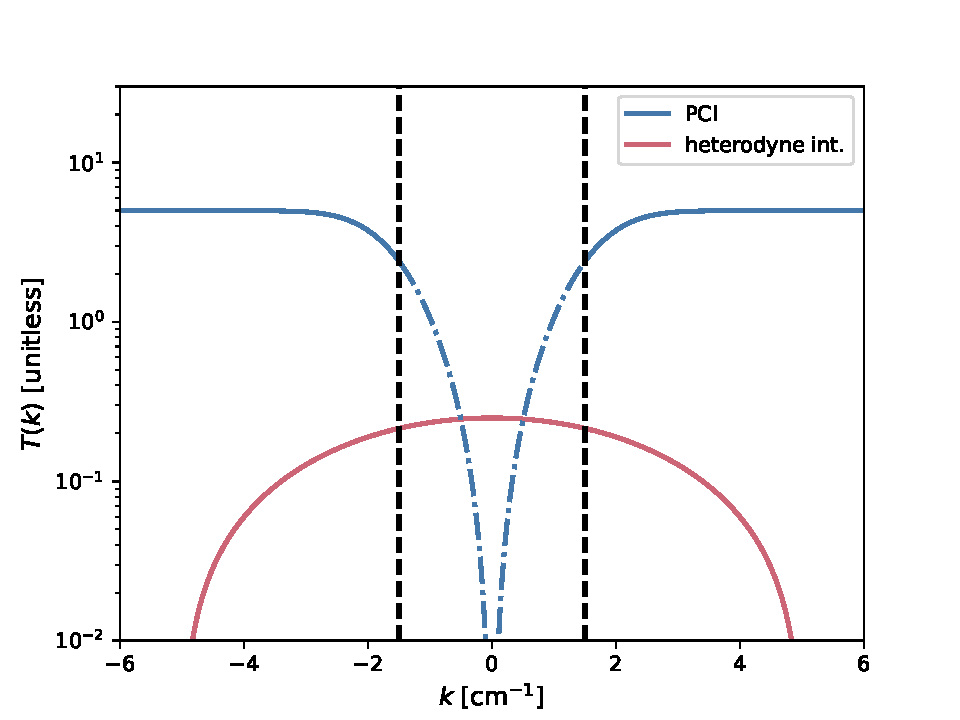
\includegraphics[width = \textwidth]{%
    Chapters/Implementation/figs/transfer_function_comparison.pdf}
  \caption[Design-point wavenumber transfer functions of combined PCI-interferometer]{%
    The design-point wavenumber transfer function
    of the heterodyne interferometer relative to
    that of the pre-existing PCI system.
    The heterodyne interferometer can detect fluctuations from
    $k = 0$ up to its finite sampling-volume cutoff
    (\ref{eq:Implementation:kfsv_interferometer_design}).
    The vertical, dashed lines indicate
    the low-$k$ cutoff of the PCI phase-plate groove,
    $k_g$ from (\ref{eq:Implementation:kg_realized});
    the phase-plate high-$k$ cutoff (\ref{eq:Implementation:kD}) and
    the PCI finite sampling-volume cutoff (\ref{eq:Implementation:kfsv_pci})
    are sufficiently large to negligibly affect the PCI transfer function
    over the depicted wavenumber domain.
    The reflectivity of the PCI phase groove is $\eta = 0.17$.
    Because the PCI transfer function is not defined for $|k| \lesssim k_g$,
    the low-$k$ PCI amplitude response
    (\ref{eq:InterferometricMethods:PCI_amplitude_response})
    is indicated by the dash-dot curves instead.
    The depicted transfer functions should be compared
    to those without finite sampling-volume effects in
    Fig.~\ref{fig:InterferometricMethods:interferometric_method_transfer_functions}.
  }
\label{fig:Implementation:transfer_function_comparison}
\end{figure}


\subsection{Detector-element size}
The heterodyne interferometer's design-point finite sampling-volume cutoff
(\ref{eq:Implementation:kfsv_interferometer_design})
fixes the ratio
of the imaging system's (absolute) magnification $|M|$
to the detector element's linear size $s_x$.
Commercially available detector elements for use at $\SI{10.6}{\micro\meter}$
range in linear size from fractions of a millimeter
to several millimeters~\cite{vigo_catalog}.
Smaller linear element size $s_x$ eases both
the beam-coalignment constraint
(\ref{eq:DesignConsiderations:summary:coalignment_constraint}) and
the curvature-matching constraint
(\ref{eq:DesignConsiderations:summary:radii_of_curvature_matching}).
The variation of detector noise and shot noise
with $s_x$ (but fixed $M / s_x$) can also be examined.
\graffito{\textcolor{red}{Why make this assumption?}}
To proceed, assume that the interferometer image plane
sits in the corresponding Rayleigh range
(i.e.\ $|z_{\image}| \ll z_R$) such that
$w(z_{\image}) \approx |M| w_{\object}$, where
$w(z_{\image})$ is the 1/e $E$ radius of the probe beam at the image plane, and
$w_{\object}$ is the 1/e $E$ radius of the probe beam at the object plane.
The optical power of the probe beam impinging on the detector element is
a function of $s_x / w(z_{\image})$, i.e.\
$P_P = P_P(s_x / w(z_{\image})) \approx P_P(s_x / (|M| w_{\object}))$;
because $M / s_x$ is fixed by the design-point finite sampling-volume cutoff
(\ref{eq:Implementation:kfsv_interferometer_design}),
$P_P$ is also approximately fixed.
The optical power in the reference beam impinging on the detector element,
however, is independent of the magnification and
proportional to the element area $A$, i.e.\ $P_R \propto A$.
Thus, the one-sided autospectral density
of the demodulated detector noise
(\ref{eq:DesignConsiderations:summary:detector_noise_autospectral_density})
is \emph{independent} of the element size.
The one-sided autospectral density
of the demodulated shot noise
(\ref{eq:DesignConsiderations:summary:shot_noise_autospectral_density})
is, in general, a function of the element size;
in the extreme $P_R \gg P_P$,
the spectral density is \emph{independent} of the element size;
in the opposite extreme $P_R \ll P_P$,
the spectral density varies inversely with element area $A$.
In light of the above considerations,
a square detector element of intermediate linear size
\begin{equation}
  s_x = \SI{1}{\milli\meter}
  \label{eq:Implementation:detector_size}
\end{equation}
was chosen.
Referencing the definition of the finite sampling-volume cutoff
(\ref{eq:DesignConsiderations:summary:finite_sampling_volume_cutoff}) and
the interferometer's corresponding design point
(\ref{eq:Implementation:kfsv_interferometer_design}),
it naturally follows that the interferometer imaging system
must have magnification
\begin{equation}
  |M| = 0.08.
  \label{eq:Implementation:magnification_interferometer_design}
\end{equation}


\subsection{Beam coalignment in presence of machine vibrations}
\label{sec:Implementation:OpticalLayout:coalignment_with_feedback}
\diiid's PCI system has an elaborate feedback control system
that dynamically centers the unscattered beam on the phase-plate groove
\cite[Sec.~3.5]{coda_phd}.
Coda has extensively characterized the effect of this feedback system
on the lateral position of the PCI image~\cite[Sec.~3.5(f)]{coda_phd}.
This section extends Coda's analysis by examining
the effect of the feedback system on the misalignment angle $\theta$
between the unscattered probe beam and the image-plane optical axis.
It readily follows from this discussion that,
for certain imaging systems,
the PCI feedback system can dynamically maintain
the beam coalignment
(constraint (\ref{eq:DesignConsiderations:summary:coalignment_constraint}))
of a heterodyne interferometer in the presence of machine vibrations.

First, consider the situation without feedback.
Let the probe beam propagate a distance $l$
from the plasma midplane to a focusing optic with focal length $f$, and
let the focused beam come to a waist a distance $l'$ from the focusing optic.
Now, let a single mirror,
located a distance $d$ upstream from the focusing optic,
be titled away from its nominal position (e.g.\ from machine vibrations),
deflecting the unscattered beam by angle $\beta_1$
relative to the nominal optical axis.
The resulting focal-plane position and orientation of this beam are incorrect
(i.e.\ the beam does not lie on the optical axis, but it should).
This misalignment is depicted by the solid line in
Fig.~\ref{fig:Implementation:feedback_effects}(a).
In a perfectly aligned system,
the focal-plane position and orientation of this beam
would correspond to the ``effective'' beam path
depicted by the dashed line in
Fig.~\ref{fig:Implementation:feedback_effects}(a).
The imaging optics image the object-plane ray
corresponding to this effective beam path.

\begin{figure}
  \centering
  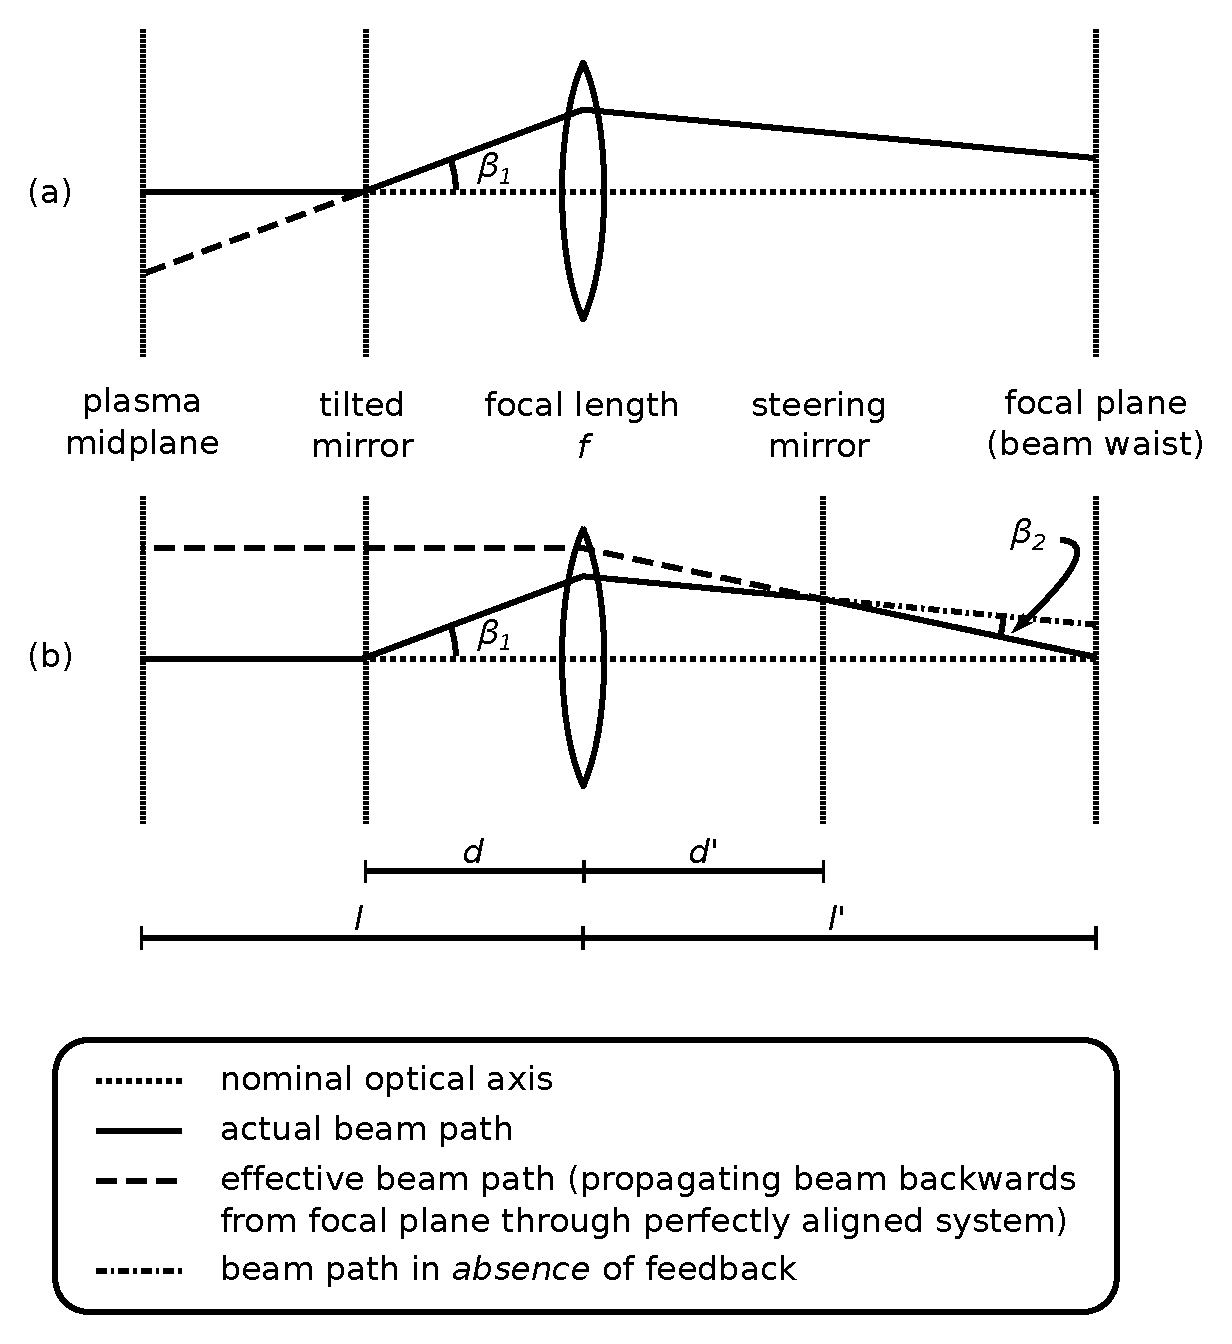
\includegraphics[width = 0.85 \textwidth]{%
    Chapters/Implementation/figs/feedback_effects.pdf}
  \caption[Effect of focal-plane feedback on imaged radiation]{%
    Effect of a tilted mirror
    (a) without focal-plane feedback and
    (b) with focal-plane feedback
    on the actual and effective paths of a Gaussian beam.
    An imaging system images the object-plane ray
    corresponding to the effective beam path.
    Without focal-plane feedback,
    both the transverse distance and the angular orientation
    of the effective object-plane ray are incorrect,
    producing errors in the corresponding image-plane quantities.
    With focal-plane feedback, however,
    the angular orientation of the effective object-plane ray is corrected
    (i.e.\ the ray is parallel to the optical axis,
    albeit laterally displaced);
    then, if the imaging system is engineered
    such that $C = 0$ in the $ABCD$ ray matrix,
    the feedback will dynamically maintain
    the correct angular orientation of the corresponding image-plane ray.
  }
\label{fig:Implementation:feedback_effects}
\end{figure}

Imaging systems are discussed in
Appendix~\ref{app:ImagingSystems}, but
the relevant details are briefly summarized here.
The symmetry axis of a Gaussian beam
behaves as a ray in the geometric-optics sense, where
a ray is fully described by
its transverse distance $\rho$ to the optical axis and
its angular orientation $\theta$ relative to the optical axis.
Ray propagation through a magnification-$M$ imaging system
is well-characterized by an $ABCD$ ray matrix of the form
(\ref{eq:ImagingSystems:ABCD_imaging}).
Specifically,
\begin{align}
  \rho_{\image} &= M \rho_{\object},
  \\
  \theta_{\image} &= \frac{\theta_{\object}}{M} + C \rho_{\object},
\end{align}
where $\object$ indicates object-plane quantities,
$\image$ indicates image-plane quantities, and
$C$ is constant determined by the particulars of the imaging system.
In a perfectly aligned system,
the unscattered beam's object-plane ray
($\rho_{\object} = 0$ and $\theta_{\object} = 0$)
is correctly imaged as $\rho_{\image} = 0$ and $\theta_{\image} = 0$.
However, in a \emph{misaligned} system,
the unscattered beam's \emph{effective} object-plane ray
($\rho_{\object} \neq 0$ and $\theta_{\object} \neq 0$)
is imaged as $\rho_{\image} \neq 0$ and $\theta_{\image} \neq 0$.
Thus, without feedback, a tilted mirror
produces errors in both the image-plane position and orientation
of the unscattered beam.

Now, add a steering mirror a distance $d'$ downstream of the focusing optic.
This steering mirror is tasked with compensating for the titled mirror
by returning the unscattered beam's focal-plane position
to the nominal optical axis,
as depicted in Fig.~\ref{fig:Implementation:feedback_effects}(b).
In the geometric-optics limit,
a ray passing through the intersection of
the optical axis and the focal plane
corresponds to a collimated beam ($\theta = 0$)
upstream of the focusing optic.
Thus, in a perfectly aligned system,
the focal-plane position and orientation
of the feedback-compensated beam
would correspond to the ``effective'' beam path,
depicted by the dashed line in
Fig.~\ref{fig:Implementation:feedback_effects}(b).
Thus, upstream of the focusing optic,
the effective beam path is displaced from but \emph{parallel}
to the nominal optical axis.
As is the case without feedback,
the imaging optics image the object-plane ray
($\rho_{\object} \neq 0$, $\theta_{\object} = 0$)
corresponding to this effective beam path, i.e.\
$\rho_{\image} = M \rho_{\object}$ and
$\theta_{\image} = C \rho_{\object}$.
Thus, for imaging systems with $C = 0$,
the PCI feedback system
will dynamically maintain the correct angular orientation
of the image-plane unscattered beam
(i.e. $\theta_{\image} = 0$);
an obvious application is satisfying
the heterodyne interferometer's coalignment constraint
(\ref{eq:DesignConsiderations:summary:coalignment_constraint})
in the presence of machine vibrations.
Of course, the lateral shifts in image location
documented by Coda~\cite[Sec.~3.5(f)]{coda_phd}.


\subsection{Reference-beam generation}
\label{sec:Implementation:OpticalLayout:reference_beam_generation}
A heterodyne interferometer interferes the imaged probe radiation
with a frequency-shifted reference beam
to make an absolute phase measurement, as discussed in
Section~\ref{sec:InterferometricMethods:interferometry:heterodyne}.
It is easy to Doppler shift $\SI{10.6}{\micro\meter}$ radiation
by tens of $\SI{}{\mega\hertz}$ with an acousto-optic modulator (AOM).
The operation of a typical AOM is described in
in Section~\ref{sec:DesignConsiderations:phase_noise:LO}.

The heterodyne interferometer's reference beam is generated
with a Gooch \& Housego (Ilminster, UK) 37027-5 Germanium AOM,
pictured in Fig.~\ref{fig:Implementation:aom}.
The resonant frequency of the AOM's piezo-actuator
is $\SI{27.12}{\mega\hertz}$, but
the AOM's deflection efficiency varies negligibly
between $\SI{25}{\mega\hertz}$ and $\SI{30}{\mega\hertz}$.
\graffito{\textcolor{red}{As will be discussed\ldots operate at $\SI{30}{\mega\hertz}$}}
For operation at $\Delta f_0 = \SI{30}{\mega\hertz}$,
the deflected beam is separated from the undeflected beam by
$2 \theta_B = \SI{59}{\milli\radian}$, where
$\theta_B$ is the Bragg angle from
(\ref{eq:DesignConsiderations:Bragg_angle}).
Deflection efficiency scales roughly linearly with RF power, and
deflection efficiencies in excess of $75\%$
can be obtained at the maximum-rated RF power of $\SI{30}{\watt}$.
The RF power is CW such that
the AOM simply deflects and Doppler shifts
a fraction of the incident optical beam.
(In contrast, rapidly varying the RF power modulates
the optical powers in the deflected and undeflected beams, but
such modulation is \emph{not} desirable in a heterodyne interferometer).
The AOM's static optical insertion loss is $\leq 15\%$, and
the incident optical intensity should be limited to
$\leq \SI{5}{\watt\per\milli\meter\squared}$
to avoid thermal lensing of the beam.
The diameter of the piezo-driven acoustic beam is $\sim\SI{5}{\milli\meter}$.
Satisfying both the AOM's peak-intensity constraint and
the aperture-diffraction constraint
(\ref{eq:DesignConsiderations:summary:aperture_radius_for_minimal_diffraction},
with the acoustic beam providing an ``effective aperture'')
requires placement of the AOM $\sim15"$ downstream
of the laser's beam waist.
\graffito{\textcolor{red}{Need a section on source parameters}}

\begin{figure}
  \centering
  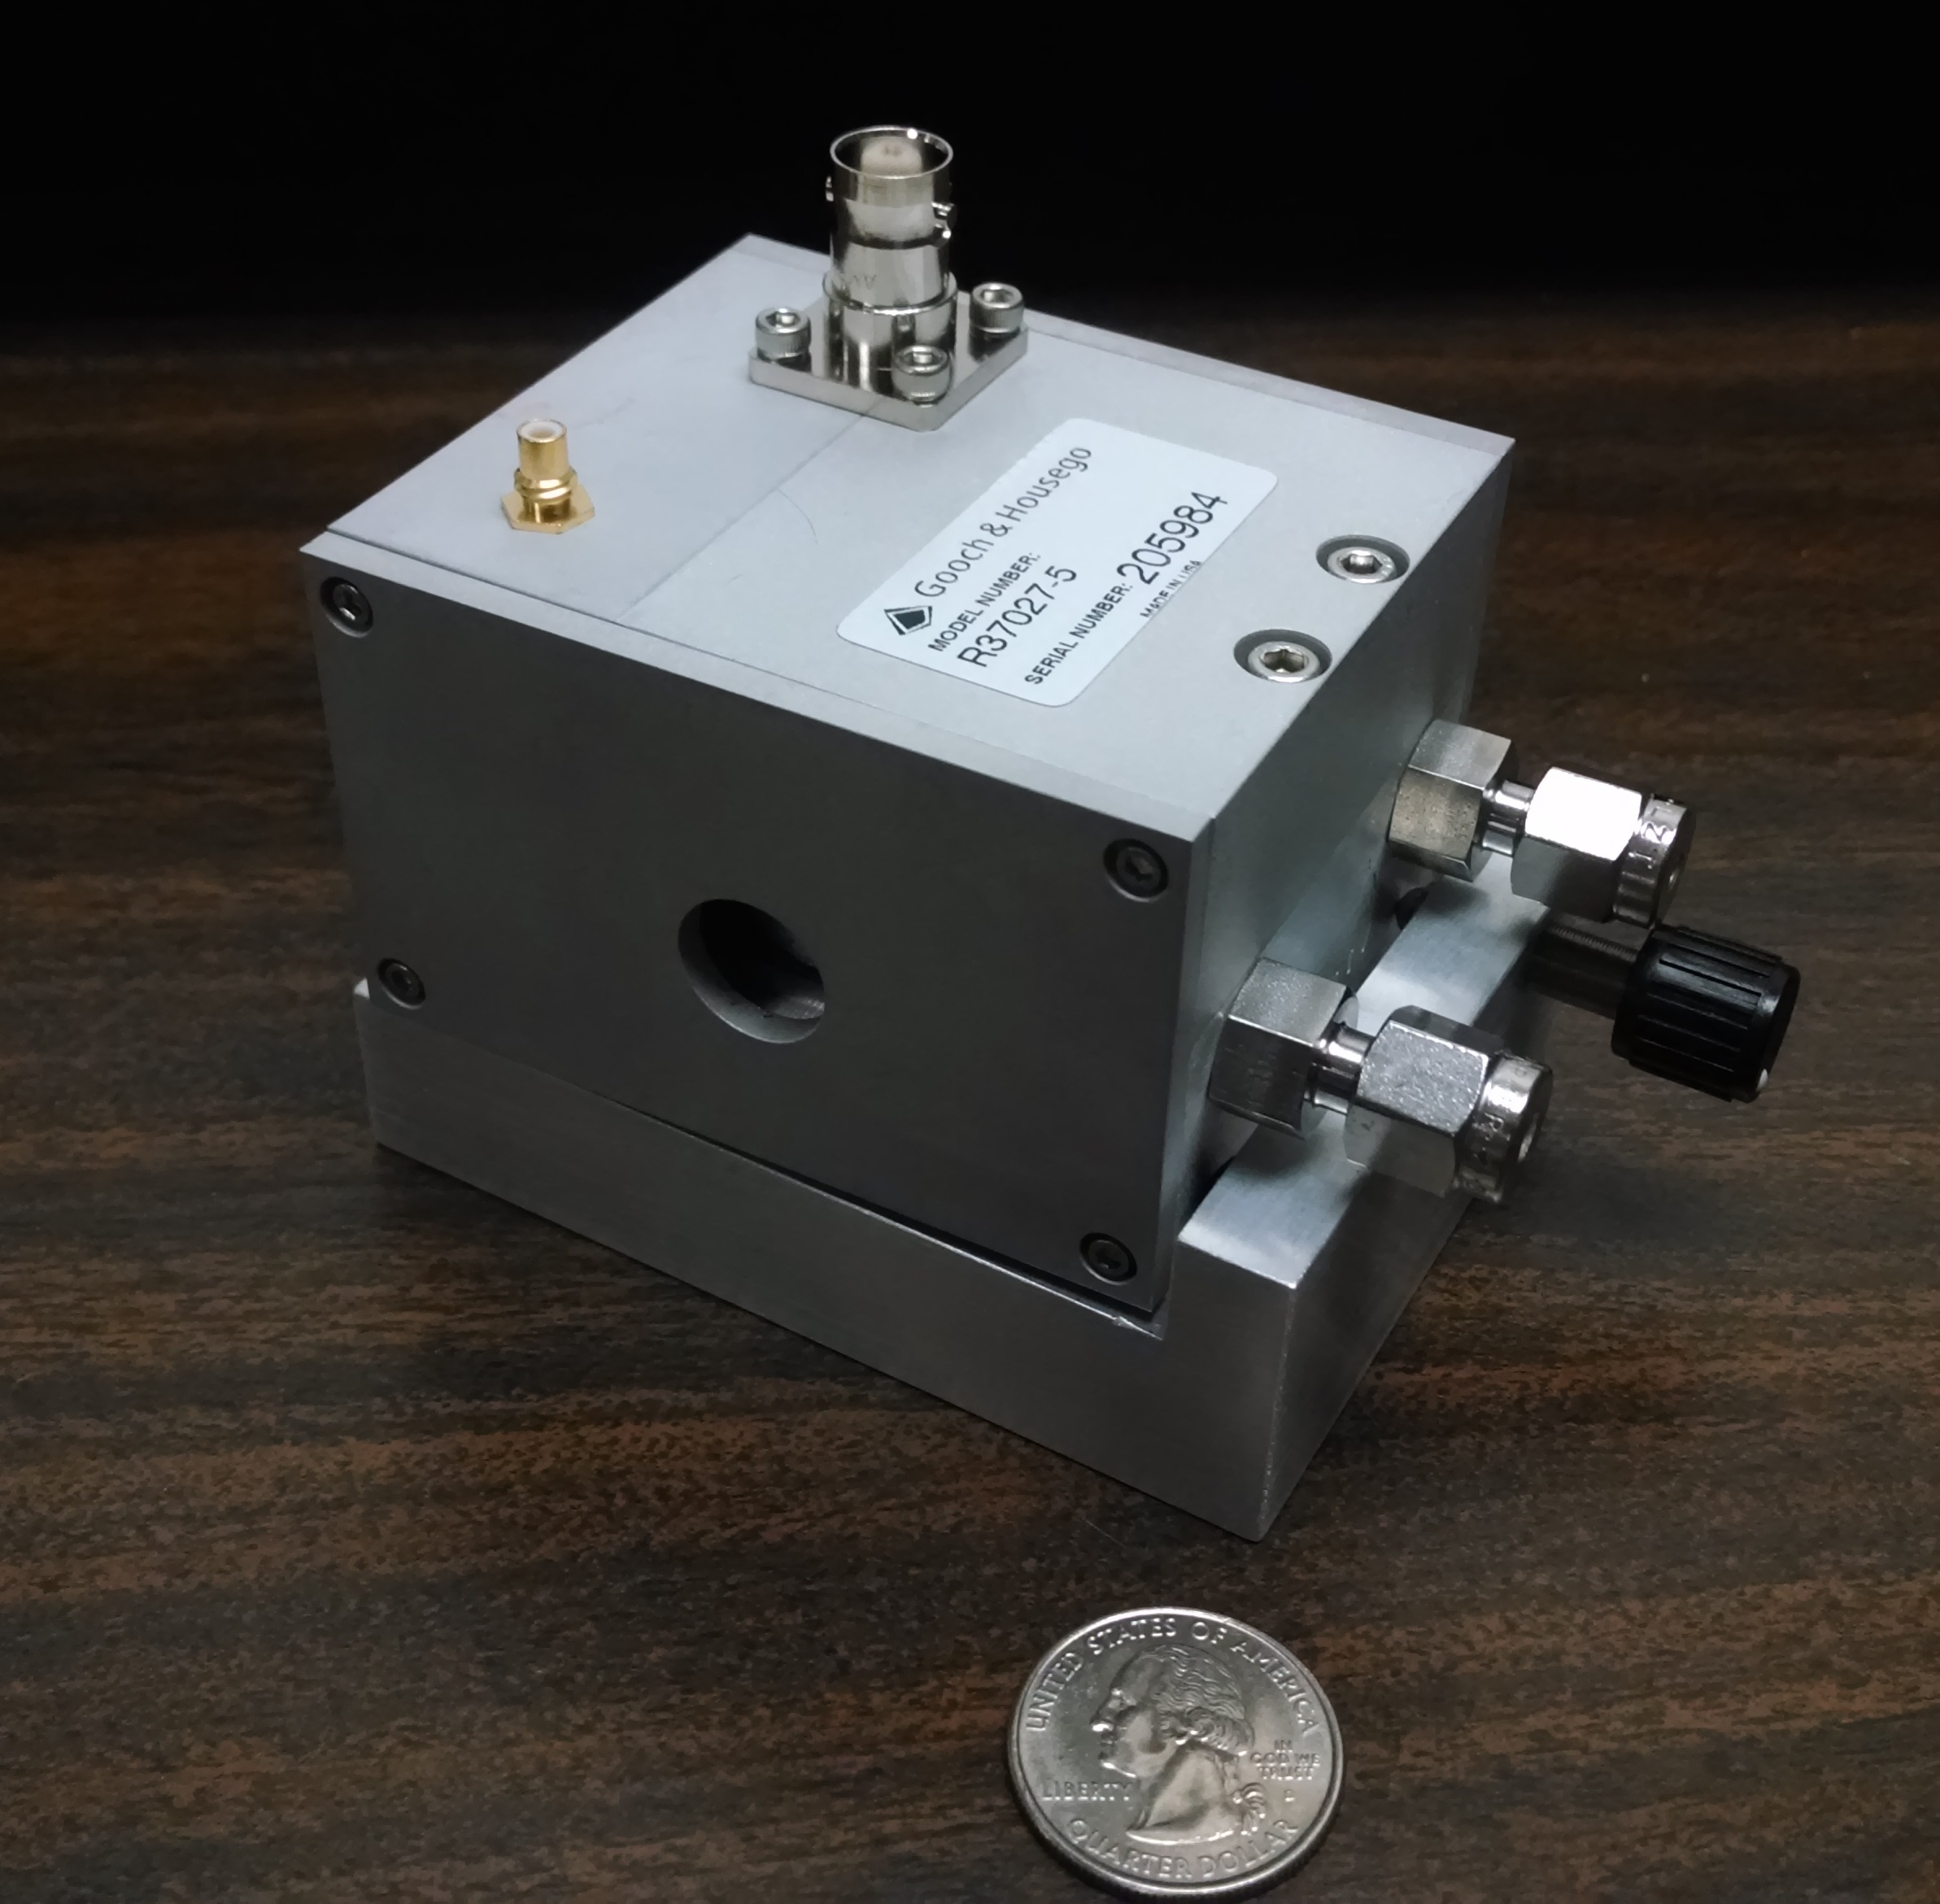
\includegraphics[width = 0.6 \textwidth]{%
    Chapters/Implementation/figs/aom.jpg}
  \caption[Acousto-optic modulator (AOM)]{%
    The heterodyne interferometer's Germanium acousto-optic modulator (AOM).
    The AOM deflects and Doppler shifts ($\Delta f_0 = \SI{30}{\mega\hertz}$)
    a fraction of the incident CO$_2$ beam ($f_0 = \SI{28.3}{\tera\hertz}$)
    to produce a reference beam.
    The $\SI{30}{\mega\hertz}$ RF signal is coupled to the AOM
    through the upper-left BNC jack, and
    the resulting sound waves propagate through the Germanium crystal
    from left to right.
    The CO$_2$ beam enters through the aperture on the AOM's face and
    exits through a similar aperture on the AOM's rear.
    The twin Swagelock fittings on the AOM's right
    provide an inlet and outlet for water cooling, while
    the lower-left SMC jack connects to
    a normally closed, creep-action PEPI N thermostat
    that provides a thermal interlock to the AOM's RF driver.
    The AOM is mounted on a ``Bragg mount'', which
    allows easy optimization of the beam's angle of incidence
    (via the mount's adjustment screw, seen in black at the middle-right).
  }
\label{fig:Implementation:aom}
\end{figure}

Due to space constraints, the reference-beam path length
is \emph{not} matched to the probe-beam path length.
This path-length discrepancy \textcolor{red}{$L \approx \SI{10}{\meter}$}
injects the laser's phase noise
into the heterodyne interferometer's measurements, as quantified by
(\ref{eq:DesignConsiderations:summary:laser_phase_noise_autospectral_density}).
However, as shown in \textcolor{red}{Section~???},
the laser's phase noise negligibly contributes
to the heterodyne interferometer's noise floor.

Allowing such a ``modest'' path-length discrepancy
substantially simplifies the optical design of the reference arm.
Following its generation at the AOM,
the reference beam is directed to the interferometer detector
with four broadband metallic mirrors
(ER.2 protected-silver coated from
Newport Corporation, Irvine, CA USA) and
is combined with the probe beam
via a 50\% reflective, polarization-independent ZnSe beam splitter
(II-VI Infrared, Saxonburg, PA USA).
No lenses are used to condition the reference beam.
However, a multiple-order $\SI{10.6}{\micro\meter}$ half waveplate
(II-VI Infrared, Saxonburg, PA USA)
sits between the AOM and the polarization-independent beam combiner.
As the probe beam is \emph{not} confined to a single plane,
out-of-plane mirror reflections can rotate the probe-beam polarization;
the half waveplate allows one to easily align the polarization
of the reference beam with that of the probe beam,
thereby maximizing the interference signal.
From source to detector, the reference beam
propagates a total distance $59\text{-}3/8"$.


\subsection{Probe-beam generation \& imaging}
The heterodyne interferometer and the pre-existing PCI system
\emph{share} the in-vessel probe beam.
The only modification to the beam-generation optics
was the addition of the AOM, discussed extensively in
Section~\ref{sec:Implementation:OpticalLayout:reference_beam_generation}.
The AOM insertion loss and
the diversion of some of the laser power to the reference arm
reduce the power in the probe beam relative to the PCI-only configuration.

As in the PCI system, the probe arm of the heterodyne interferometer
is configured to \emph{image} the probe radiation from the tokamak midplane.
The heterodyne interferometer and PCI imaging optics share
the focusing $f = 80.7"$ off-axis parabolic mirror and
the feedback steering mirrors~\cite[Sec.~3.5]{coda_phd}.
Because the phase plate's spatial filtering
produces the PCI's low-$k$ cutoff,
a $2"$ diameter $S$-polarization ZnSe splitter
(II-VI Infrared, Saxonburg, PA USA)
located $5\text{-}1/8"$ upstream of the phase plate
diverts a fraction of the probe radiation
to dedicated heterodyne-interferometer optics.
\graffito{\textcolor{red}{What fraction??}}
(This beam splitter also diverts a portion of the unscattered probe beam
to the feedback system's quadrant detector;
the heterodyne interferometer's probe beam and
the feedback beam are separated with
an additional $2"$ diameter $S$-polarization ZnSe splitter).
Four broadband metallic mirrors
(ER.2 protected-silver coated from
Newport Corporation, Irvine, CA USA)
direct the probe radiation through the remainder
of the heterodyne interferometer's imaging optics, which
consist of two plano-convex ZnSe lenses
(II-VI Infrared, Saxonburg, PA USA).
The first lens $L1$ has a $7.5"$ focal length and a $2"$ diameter, and
the second lens $L2$ has a $7.5"$ focal length and a $1.5"$ diameter.
Then, under the constraint of imaging the plasma midplane,
the remaining design parameters are
the distance $d_{P2,L1}$ between
the focusing off-axis parabolic mirror and $L1$ and
the distance $d_{L1,L2}$ between $L1$ and $L2$.
The sensitivity of the heterodyne-interferometer optical layout
to $d_{P2,L1}$ and $d_{L1,L2}$ is shown in
Fig.~\ref{fig:Implementation:optical_design_sensitivity}.

\begin{figure}[h!]
  \centering
  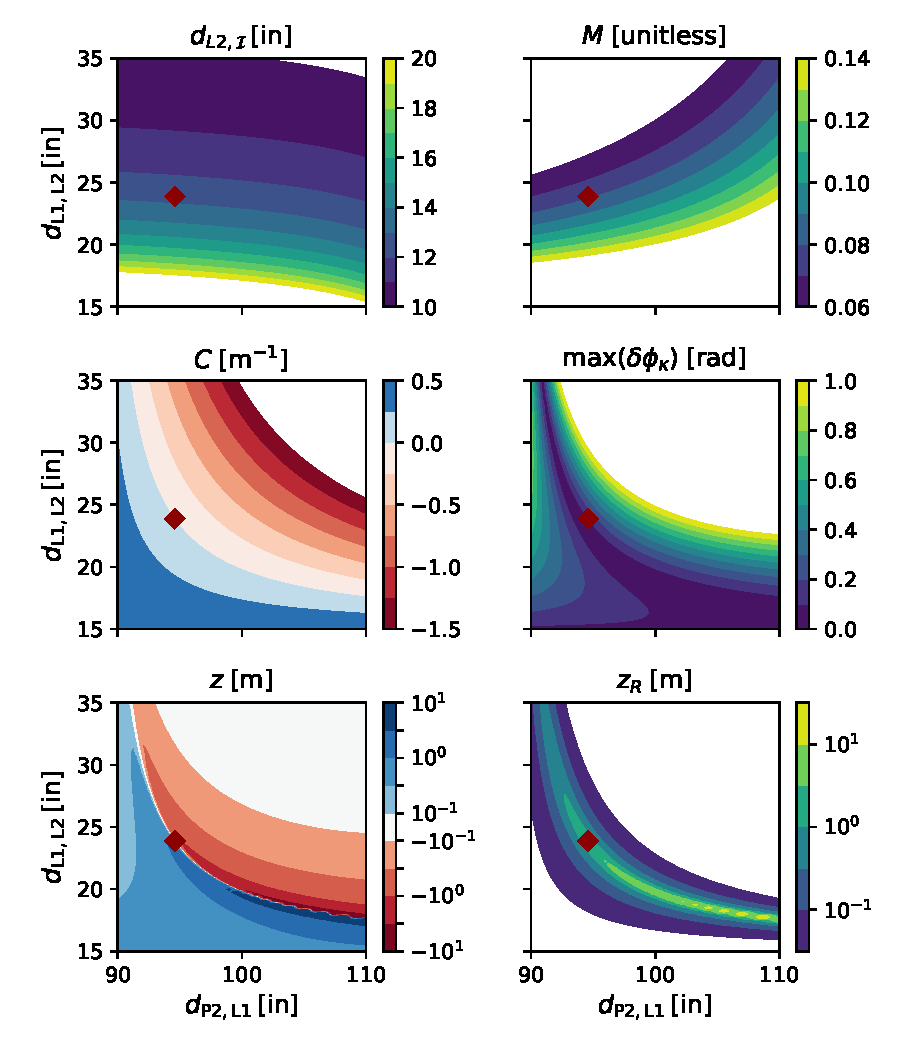
\includegraphics[width = \textwidth]{%
    Chapters/Implementation/figs/optical_design_sensitivity.pdf}
  \caption[Sensitivity of heterodyne-interferometer optical design]{%
    Sensitivity of heterodyne-interferometer optical design
    to the placement of lenses $L1$ and $L2$.
    The distance between the off-axis parabolic mirror $P2$
    (which focuses the collimated probe beam) and
    the first lens $L1$ of the imaging system
    is denoted by $d_{P2,L1}$ (along the $x$-axis), and
    the distance between $L1$ and the second lens $L2$
    is denoted by $d_{L1,L2}$ (along the $y$-axis).
    The design point is marked with a burgundy diamond.
    (Top left): Distance of image plane from $L2$
    (the detector is nominally placed at the image plane,
    inspiring the notation $d_{L2,\text{det}}$).
    (Top right): Imaging system's magnification $M$,
    with the design point in accordance with
    (\ref{eq:Implementation:magnification_interferometer_design}).
    (Middle left): Imaging system's $ABCD$ ray-matrix parameter $C$.
    As discussed in Section~\ref{sec:Implementation:OpticalLayout:coalignment_with_feedback},
    the PCI feedback system will dynamically maintain
    the coalignment of the heterodyne interferometer's beams if $C = 0$.
    (Middle right): The maximum curvature-induced phase shift
    (\ref{eq:DesignConsiderations:summary:radii_of_curvature_matching})
    for a single, $\SI{1}{\milli\meter\squared}$ square detector.
    (Bottom left): The axial distance $z$ from the image plane
    to the waist of the probe beam.
    (Bottom right): The Rayleigh range $z_R$ of the image-plane probe beam.
    A Gaussian beam has minimum radius of curvature
    $\text{min}(R(z)) = 2 z_R$; according to
    (\ref{eq:DesignConsiderations:summary:depth_of_focus_wavenumber_distortion}),
    then, there will be minimal wavenumber distortion
    if the detector is $|\delta z_{\image}| \ll 2 z_R$
    within the image plane.
  }
\label{fig:Implementation:optical_design_sensitivity}
\end{figure}

\begin{itemize}
  \item Describe resulting parameters (?)
  \item Talbot effect plot?
  \item Plot of unscattered \& scattered beam through imaging system
  \item List/table of interferometer and reference-arm layout (?)
    \begin{itemize}
      \item Difference in optical path length
      \item Plots of probe beam and scattering??
    \end{itemize}
\end{itemize}


\section{Interferometer design study}


\subsection{Expected noise}

\begin{itemize}
  \item Demodulated NEP from
    (\ref{eq:DesignConsiderations:demodulated_NEP_spectral_density}) gives
    $\sim \SI{e-18}{\watt\squared\per\hertz}$
  \item Demodulated shot noise from
    (\ref{eq:DesignConsiderations:demodulated_shot_noise_spectral_density})
    gives $\sim \SI{e-21}{\watt\squared\per\hertz}$
\end{itemize}


\section{Interferometer component selection}
\subsection{Acousto-optic modulator}
\subsection{Imaging optics}
\subsection{Detector}
\subsection{Electronics}
\begin{itemize}
  \item Automatic gain-control amplifier
  \item Analog I/Q demodulator
  \item Low-frequency ``audio'' amplifiers
\end{itemize}
\subsection{Digitizer}
\begin{itemize}
  \item Bit noise
\end{itemize}




\section{Fighting phase noise}
\subsection{Local oscillator stability}


\section{Sound-wave calibration of combined PCI-interferometer}
\subsection{Sound-wave characterization}
\subsection{Measurements}
\begin{itemize}
  \item Wavenumber range
  \item Cross calibration
  \item System sensitivity
\end{itemize}

\begin{table}[ht]
  \centering
  \renewcommand{\arraystretch}{1.5}% Spread rows out...
  \begin{tabular}{%
    >{\centering}m{3.0cm} >{\centering}m{4.5cm} >{\centering}m{4.5cm}
  }
    \toprule%
    \textbf{Parameter} & \textbf{PCI} & \textbf{Interferometer}
    \tabularnewline%
    \midrule
    \textbf{probe beam} & single CO$_2$ beam & single CO$_2$ beam
    \tabularnewline%
    \textbf{frequency bandwidth}
    & \SI{10}{\kilo\hertz} $ < f < $ \SI{2}{\mega\hertz}
    & \SI{10}{\kilo\hertz} $ < f < $ \SI{2}{\mega\hertz}
    \tabularnewline%
    \textbf{spatial bandwidth}
    & \SI{1.5}{\centi\meter}\ts{-1} $ < k < $ \SI{20}{\centi\meter}\ts{-1}
    & \SI{0}{\centi\meter}\ts{-1} $ < k < $ \SI{5}{\centi\meter}\ts{-1}
    \tabularnewline%
    \toprule%
  \end{tabular}
  \caption[Parameters of \diiid's combined PCI-interferometer]{%
    PCI and interferometry have compatible probe beams, comparable
    frequency bandwidths, and \emph{complementary} spatial bandwidths.
    All parameters are for DIII-D's currently implemented PCI--interferometer
    system.
  }%
\label{table:Implementation:PCI_interferometer}
\end{table}


\section{Looking towards ITER\ldots}


\section{Component replacement}
Over the course of this work,
several components crucial to the operation of the PCI
(and the soon-to-be-described interferometer)
failed.
The failures and replacements are briefly described below.


\subsection{Quadrature detector for beam-position feedback}
A quadrature detector measures the position
of the unscattered beam on the phase plate,
providing the input to the feedback control system
that dynamically centers the unscattered beam
on the phase-plate groove~\cite[Sec.~3.5]{coda_phd}.
As the quadrature detector
cannot physically be co-located with the phase plate,
a beam splitter samples the unscattered beam
immediately upstream of the phase plate, and
a single lens \emph{images} onto the quadrature detector
the point in the sampled beam that corresponds to the phase-plate location.
Thus, beam movement on the phase plate is mirrored
by movement of the sampled beam on the quadrature detector.
System response is maximized
with imaging magnification $|M| \approx 1$
(relative to the beam size at the phase plate) and
incident optical intensities $I_{\text{opt}}$
well beyond the linear saturation intensity
(i.e. $I_{\text{sat}} \ll I_{\text{opt}} < I_{\text{dam}}$)
~\cite{marinoni_FB_detector_report}~\cite[Sec.~3.5(b)]{coda_phd}.

The old quadrature detector consisted of four
photoconductive, liquid-nitrogen cooled, HgCdTe elements.
Quadrature detectors for use at $\SI{10.6}{\micro\meter}$
had only just become commercially available
when this unit was procured from Belov Technology in the mid-1990s
~\cite[Sec.~3.5(b)]{coda_phd}.
Cooling HgCdTe can
extend the long-wavelength cutoff beyond $\SI{10.6}{\micro\meter}$,
reduces noise, and
increases responsivity~\cite{vigo_catalog}.
In particular, HgCdTe's responsivity increases by $\sim 10^3$
when cooled to liquid-nitrogen temperatures such that
that the incident optical signal
exceeds the $1 / f$ noise
characteristic of photoconductive detectors~\cite{vigo_catalog}.
As the bandwidth requirements for the PCI feedback system
extend from DC to $\lesssim \SI{10}{\kilo\hertz}$,
$1 / f$ noise cannot be easily combated by
e.g.\ mechanically chopping the beam.
After $\sim 20$ years of operation,
the old quadrature detector failed in December 2014,
presumably having reached its expected lifetime.
As Belov Technology no longer exists,
it was not possible to procure a drop-in replacement.
Fortunately, in the context of position sensing,
HgCdTe technology has significantly improved since the mid-1990s.

The new quadrature detector
(four VIGO PVM-10.6 elements mounted on a VIGO QIP preamplifier)
is in many ways superior to the old quadrature detector.
This superiority stems from VIGO's use of
``multiple heterojunction'' HgCdTe detector elements~\cite{vigo_catalog},
which endow the detector with several advantageous properties.
First, the detector is photovoltaic.
Thus, the detector is \emph{not} plagued by the $1 / f$ noise
characteristic of photoconductive detectors.
Second, the detector's long-wavelength cutoff
sits beyond $\SI{10.6}{\micro\meter}$ at room temperature.
Taken together, the above two properties imply that
the new quadrature detector can be operated at room temperature,
i.e.\ it does \emph{not} need to be cooled by liquid nitrogen.
Lacking a dewar, the new quadrature detector
is much smaller than the old quadrature detector;
the new detector can also be mounted with an arbitrary orientation,
whereas the dewar of the old detector required an upright orientation.
This new-found flexibility substantially opened
the optical design space for the feedback arm and
the plasma arm of the soon-to-be-described interferometer.
Additionally, the dewar of the old quadrature detector
only had a $\sim \SI{6}{\hour}$ hold time,
which is not sufficient for a full day of \diiid \space operations;
thus, the use of a room-temperature quadrature detector has
eliminated the mid-day ``pit runs'' to refill the quadrature detector's dewar,
allowing easier operation of the system.
Although room-temperature operation reduces
the detector's specific detectivity to
$D^* \sim \SI{e7}{\centi\meter \sqrt\hertz \per\watt}$
(roughly three orders of magnitude \emph{lower} than
that of the old quadrature detector),
the optical signal corresponds to the strong, unscattered probe beam
(as opposed to e.g.\ weak beams
scattered from small-amplitude plasma fluctuations), so
the increase in noise negligibly influences operation of the feedback system.

\begin{itemize}
  \item When was new detector acquired?
  \item \textcolor{red}{Picture}
  \item \textcolor{red}{Table of properties (?)}
\end{itemize}


\subsection{CO$_2$ laser}
The old CO$_2$ laser~\cite[Sec.~3.3]{coda_phd},
manufactured by MPB Technologies,
had been in service since
the inception of the \diiid \space PCI system in the mid-1990s.
Lasing occurred via high voltage, DC-excitation
inside of a $\SI{2}{\meter}$-long, sealed-off glass tube
to produce a TEM$_{00}$ (Gaussian) mode with linear polarization.
The laser nominally had
a $\lesssim \SI{300}{\kilo\hertz}$ frequency stability
over short time windows ($\SI{0.1}{\second}$) and
a $\lesssim \SI{3}{\mega\hertz}$ frequency stability
over longer time windows ($\SI{e3}{\second}$).
The laser's tube was replaced in late 1999
when a precipitous drop in beam power indicated imminent failure.
Following the tube's replacement,
the measured beam power consistently hovered at $\sim\SI{14}{\watt}$
for many years.
However, in early 2016, the beam power again precipitously dropped.
The laser's high voltage power supply,
which was replaced in 2005 after failing,
was tested and found to be operating nominally,
suggesting that the drop in beam power
was attributable to the laser's aging tube.
Unfortunately, MPB Technologies has abandoned its efforts in CO$_2$ lasers
and was unable to replace or repair the tube.
Third-party tube repair was investigated but
ultimately deemed unacceptable due to
the required lead times and the lack of a guaranteed repair.
Fortunately, the MPB laser continued operating, albeit at reduced power,
throughout the 2016 campaign, allowing continued diagnostic development
of the soon-to-be-described interferometer.

After an exhaustive search of the CO$_2$-laser market,
a water-cooled AL30ST CO$_2$ laser was procured
from Access Laser Company (Everett, WA) in mid-2016.
Lasing occurs via RF excitation at $\SI{40.68}{\mega\hertz}$;
RF excitation requires far-lower voltages than DC excitation,
eliminating the high-voltage safety risk and allowing more efficient lasing
\cite{he_jap83}.
As in the old MPB laser,
the lasing cavity is supported by carbon fiber rods (rather than Invar)
to mitigate any effects of the tokamak's large, ambient magnetic fields
on the laser's performance.
The laser oscillates on a TEM$_{00}$ (Gaussian) mode (spec'd $M^2 < 1.1$)
with vertical polarization (spec'd extinction ratio $1 / 897$), and
its $\SI{37}{\watt}$ power output is stable to within $\pm 1.1\%$
\cite{marinoni_AL30ST_report}.
Lasing occurs on the $P(20)$ line
of the $00^{\circ}1 \rightarrow 10^{\circ}0$ transition
to produce radiation with a vacuum wavelength of
$\lambda_0 = \SI{10.591}{\micro\meter}$.
Measurements with wavelength meter 621B
from Bristol Instruments, Inc. (Victor, NY)
indicate that the laser's wavelength stability over several seconds
is characterized by a Voigt distribution with
full width at half maximum of $\SI{0.0029}{\nano\meter}$, which
corresponds to a frequency stability (over \emph{several seconds})
of $\SI{3.8}{\mega\hertz}$ \cite{marinoni_AL30ST_report}.

In the context of measuring plasma-density fluctuations
with an external reference-beam interferometer,
the relevant metric is the laser's frequency stability
over much shorter time windows
(i.e.\ the time difference corresponding to
the difference in optical path length between
the interferometer's plasma and reference arms).
This is most easily evaluated empirically
by deploying the laser in the given interferometric system
and evaluating the corresponding phase noise.
Successive test shots,
the first with the old MPB laser and the second with the AL30ST,
show comparable phase noise (and hence frequency stability)
between the two lasers.
Thus, the AL30ST frequency stability is deemed to be sufficient
for measurement of plasma-density fluctuations
with the soon-to-be-described external reference-beam interferometer.

\begin{itemize}
  \item \textcolor{red}{Picture}
  \item \textcolor{red}{Fig. of new vs.\ old laser stability}
\end{itemize}


\subsection{In-vessel mirrors}
Two of the PCI mirrors are located
\emph{inside} of the \diiid \space vacuum vessel.
As indicated in Fig.~\ref{fig:Implementation:d3d_port_locations}(b),
the PCI probe beam enters the machine through the $285^{\circ}$ R+2 port,
reflects off of the first in-vessel mirror,
propagates vertically downwards through the machine (and the plasma),
reflects off the second in-vessel mirror, and
exits the machine through the $285^{\circ}$ R-2 port.
The in-vessel mirrors are elongated
along the axis parallel to the plane of incidence
in order to increase the mirrors' apparent surface area.
The mirrors were fabricated by Esco Optics, Inc. (Oak Ridge, NJ).
The mirrors are made of fused quartz with
a reflective aluminum surface and a protective SiO coating.

In mid-2015 the beam quality of the CO$_2$ laser and the HeNe alignment laser
after passing through the \diiid \space vessel was noted to be poor
(i.e. substantially non-Gaussian).
Numerous tests suggested that the poor beam quality was attributable
damaged in-vessel mirrors;
this hypothesis was confirmed via visual inspection
during the next manned entry of the machine.
``Drop-in'' replacements were ordered from Esco Optics
and were installed in mid-2016.
The removed, damaged mirrors are shown in
Fig.~\ref{fig:Implementation:in_vessel_mirrors}.
It is not known whether the mirrors were damaged
during e.g. plasma operations or high-temperature bakes of the vessel.

\begin{figure}
  \centering
  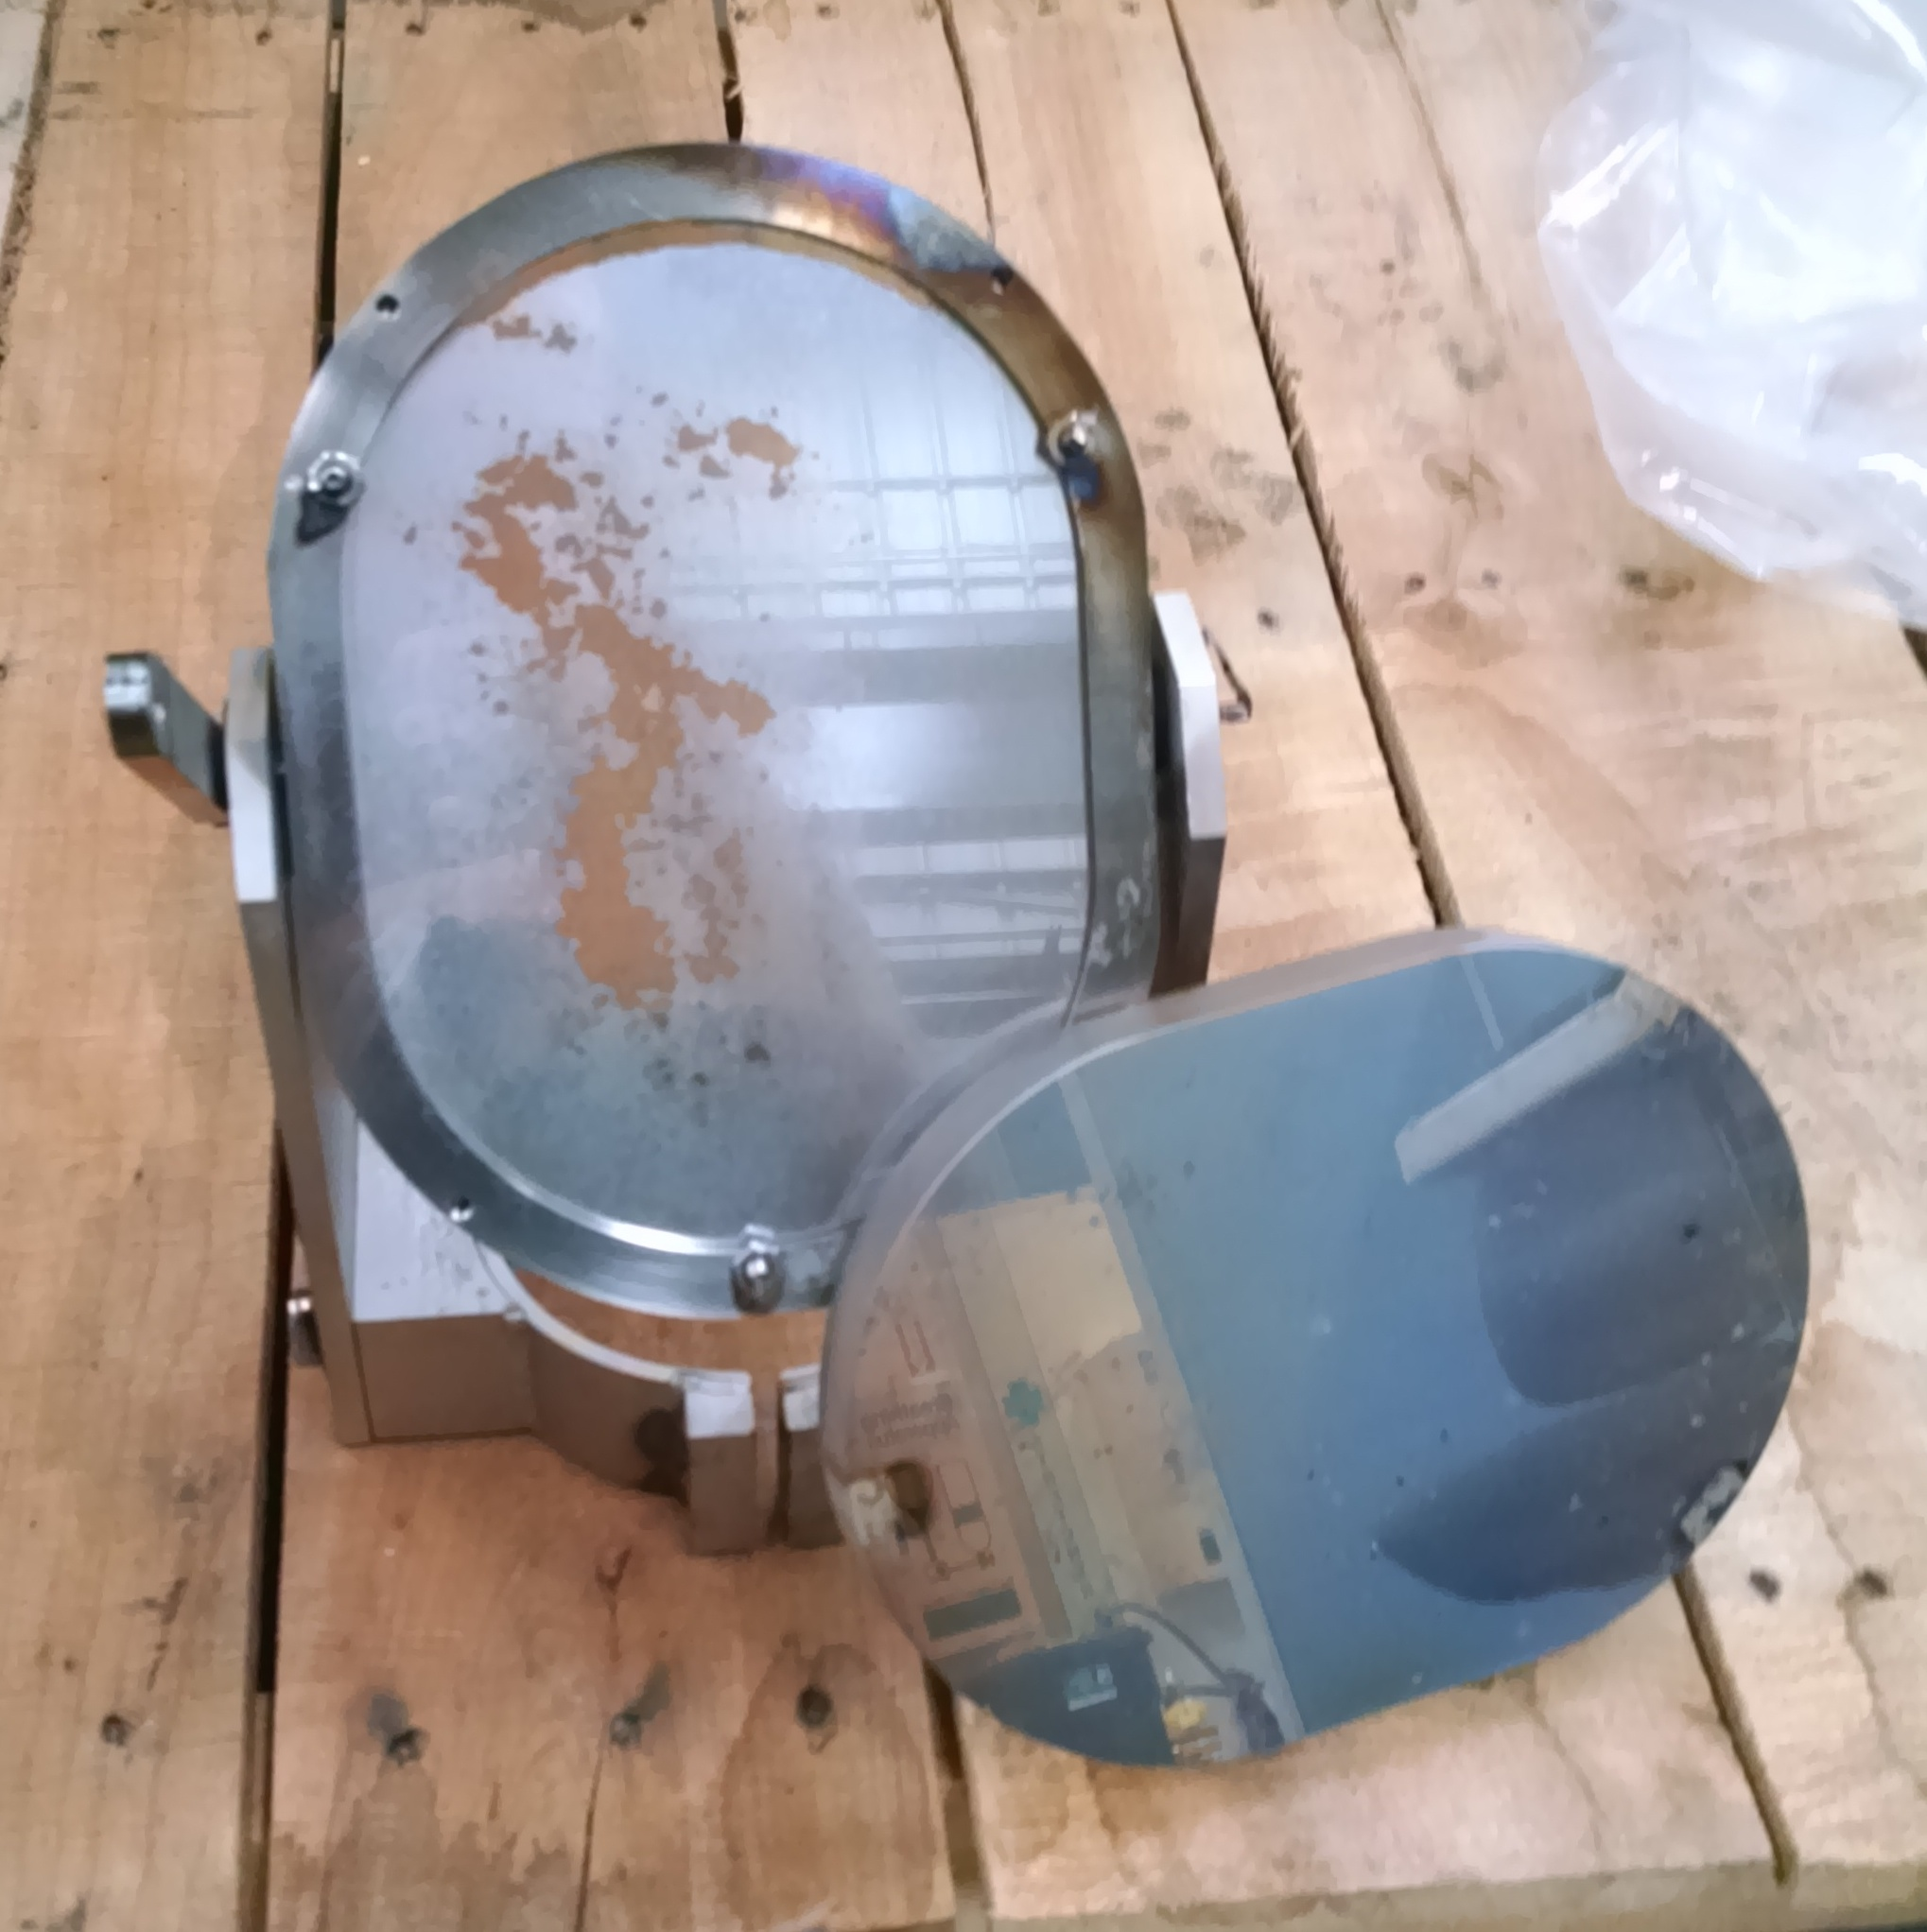
\includegraphics[width = 0.6 \textwidth]{%
    Chapters/Implementation/figs/in_vessel_mirrors.jpg}
  \caption[PCI's damaged in-vessel mirrors]{%
    PCI's damaged in-vessel mirrors, sitting
    in the \diiid \space ``Hi-Bay''
    after removal from the vessel in mid-2016.
    (Note that the reflectivity of each mirror at $\SI{10.6}{\micro\meter}$
    cannot be gauged from this photograph in the visible spectrum).
    ``Drop-in'' replacements were installed
    before the resumption of plasma operations.}
\label{fig:Implementation:in_vessel_mirrors}
\end{figure}


\bibliographystyle{plainurl}
\bibliography{references}
